\documentclass[12pt,a4paper]{article}
\renewcommand{\baselinestretch}{1.5} 
\usepackage[latin1]{inputenc}
\usepackage{amsmath}
\usepackage{amsfonts}
\usepackage{amssymb}
\usepackage{algorithm} 
\usepackage{algpseudocode} 
\usepackage{graphicx}
\usepackage{geometry}
\usepackage{tabulary}
\usepackage{caption}
\usepackage{subcaption}
\usepackage{xcolor}
\usepackage{dirtytalk}
\usepackage{bm}
\usepackage{longtable}
\usepackage{comment}
%\usepackage{ulem}
\graphicspath{{./images/}}

\usepackage[hyphens]{url}
%\usepackage{url}
% Toggle comment for hyperlinking the TOC and references
%\usepackage{hyperref}
%\hypersetup{
%	colorlinks=false%, % make the links colored
%	%linkcolor=blue, % color TOC links in blue
%	%urlcolor=red, % color URLs in red
%	%linktoc=all % 'all' will create links for everything in the TOC
%}

\geometry{
	left=2.5cm,
	right=2.5cm,
	top=2.5cm,
	bottom=3cm,
	}
	
	
	\usepackage{titlesec}
	
	\setcounter{secnumdepth}{4}
	\setcounter{tocdepth}{4}
	\titleformat{\paragraph}
	{\normalfont\normalsize\bfseries}{\theparagraph}{1em}{}
	\titlespacing*{\paragraph}
	{0pt}{3.25ex plus 1ex minus .2ex}{1.5ex plus .2ex}
	
	\newenvironment{conditions}
	{\par\vspace{\abovedisplayskip}\noindent\begin{tabular}{>{$}l<{$} @{${}={}$} l}}{\end{tabular}\par\vspace{\belowdisplayskip}}
	
	
		
\begin{document}
% uncomment title page when required to be included,
	\thispagestyle{empty}
\begin{center}
	{\Large \bf Architecture-Aware Evaluation of Range Query Processing: Mo’s Algorithm vs GPU Parallelization\\}
	
	\vspace*{0.5cm}
	{\large\textit{A Project Component for }\\}
	%\vspace*{0.3cm}
	{\large\textbf{Parallel and Distributed Computing (UCS645)}} \\
%	{\large in\\}
%	{\large \textbf{CSED} }
	
	%\vspace*{1cm}
	{\large \textit{By\\}}
	\begin{center}
	\begin{tabular}{ccc}
	\textbf{Sr} & \textbf{Name} & \textbf{Roll No}  \\
	1  & Suryansh Sharma    & 102316055 \\
	2  & Shorya Gupta     & 102316062 \\
	\end{tabular}
	\end{center}
% update the name of the students based on number
	%\vspace*{0.5cm}
		\begin{center}
                {\large \textit{Under the guidance of}}\\
					\textbf{{\large Dr. Saif Nalband}}\\
					{\large (Assistant Professor, DCSE)}\\
		\end{center} \ \\ \ \\
\begin{figure}[h]
\centering

\includegraphics[width=70mm, height=40mm]{tietlogo.jpg}
\end{figure}

%	in case the layout changes modify the below vspace 1.25 and appropiately make sure that title page is contained in one single page	
	\vspace*{0.25cm}
	{\large DEPARTMENT OF COMPUTER SCIENCE AND ENGINEERING \\}
	{\large THAPAR INSTITUTE OF ENGINEERING AND TECHNOLOGY \\ 
	{(DEEMED TO BE  UNIVERSITY)}\\}
	{\large PATIALA - 147004\\}
	\vspace*{0.3cm}
	\textbf{{\large APRIL, 2026}}
	
\end{center}

\newpage

%%%%%%%%%%%%%%%%%%%%%%%%%%%%%%%%%%%%%%%%%%
	\pagenumbering{gobble}
	\renewcommand*\contentsname{Table of Contents}
	\tableofcontents
	\newpage
	\newpage
    \listoffigures
    \newpage
    \newpage
    \listoftables
    \newpage
   % \newpage
   % \listoftables
    % \newpage
    \pagenumbering{arabic}
   
    \section{Introduction}

	\pagenumbering{arabic} 


	\subsection{Background}
	% write your Backgroud 
		Distinct elements in range queries are a fundamental primitive in analytics, indexing, and log mining. At large scales, naive per-query scans are slow and memory-inefficient, so the algorithm must be redesigned with hardware realities in mind.
		
		This project implements three architecture-aware engines: a cache-friendly single-core Mo's algorithm, a multicore SIMD OpenMP engine based on a prev-array transformation, and a CUDA kernel that assigns one warp per query.
	
	\subsection{Introduction to Problem Statement}
	Given an immutable array $A[0..N-1]$ and a set of offline range queries $[L,R]$, compute:
	\[
	\text{distinct}(L,R) = \left|\{A_i \mid L \le i \le R\}\right|
	\]
	The challenge is to answer up to $Q=100{,}000$ queries on arrays as large as $N=1{,}000{,}000$ while respecting cache locality, memory bandwidth ceilings, SIMD lane utilization, and GPU warp behavior.

	Figure \ref{fig:speedup-bar} summarizes the relative speedups at the largest workload.
		
	    \begin{figure}[h!]
			\centering
			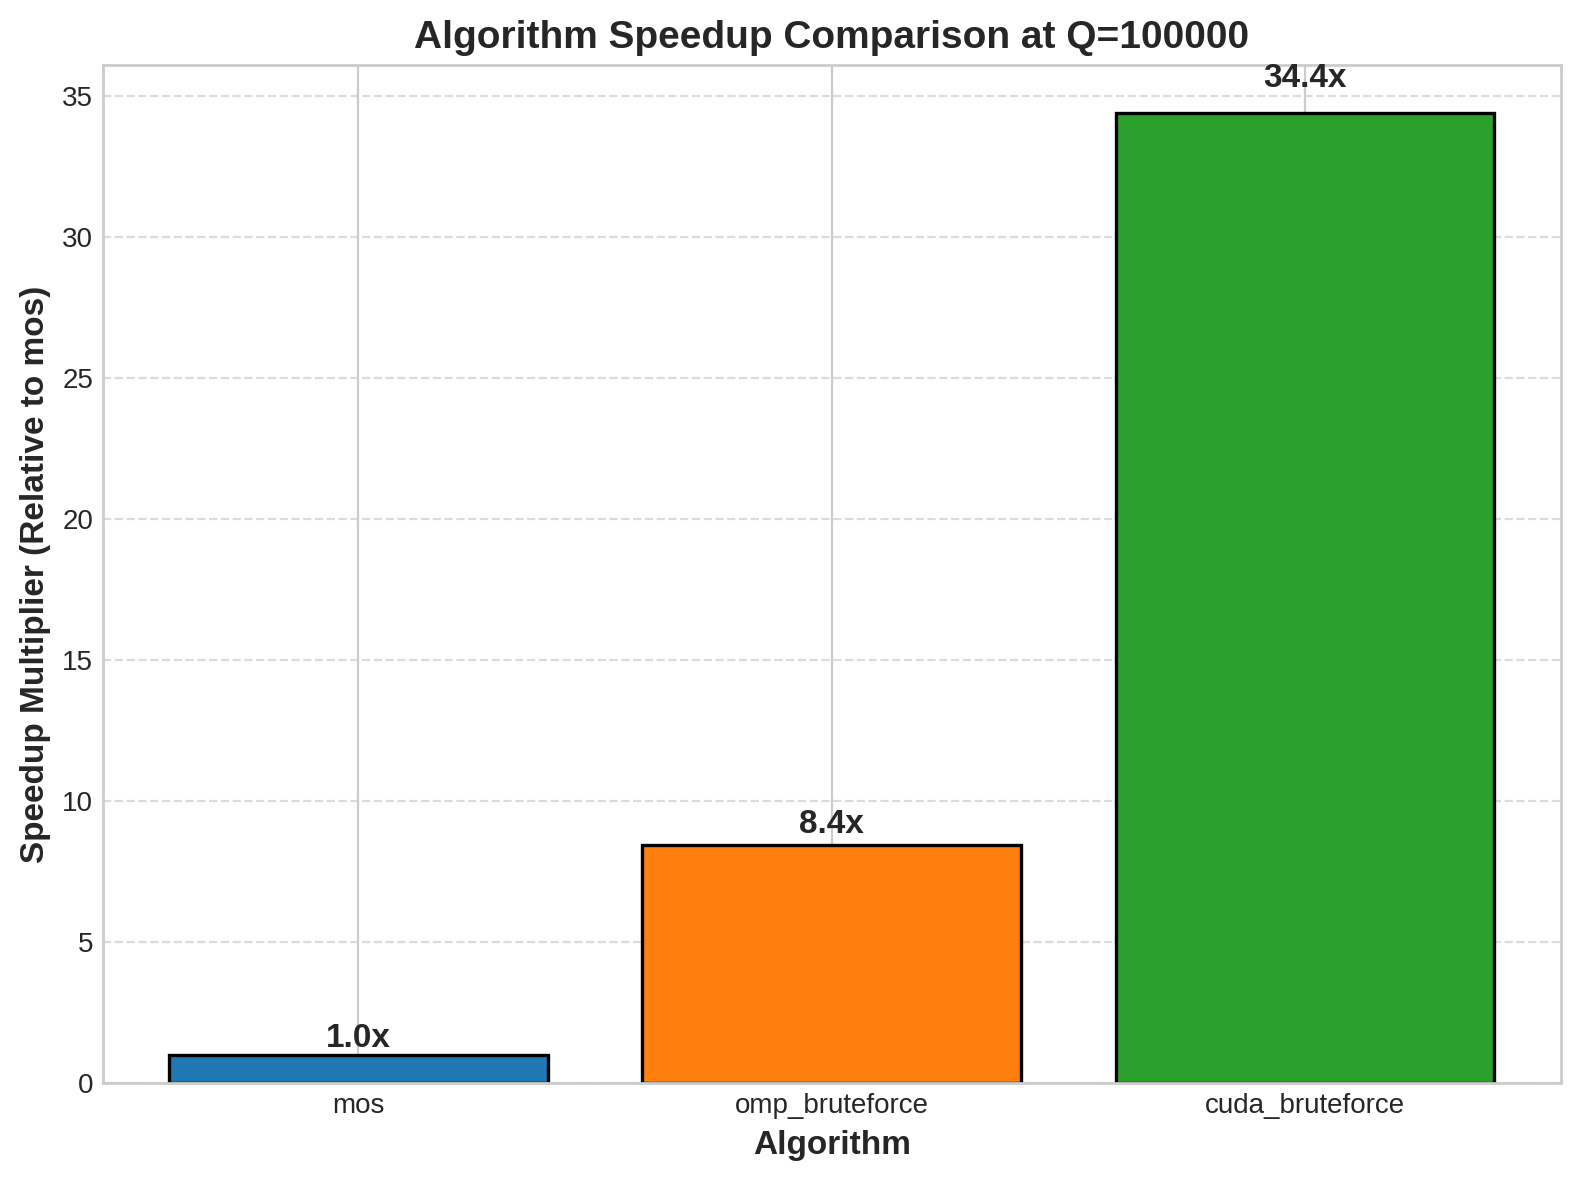
\includegraphics[width=0.85\linewidth]{plots/relative_speedup_bar.png}
			\caption{Speedup comparison at $Q=100{,}000$ (medium ranges).} 
			\label{fig:speedup-bar}
		\end{figure}
		
		Key contributions of this work are:
		\begin{itemize}
			\item Hilbert-ordered Mo's algorithm to reduce cache churn for locality-heavy query sets.
			\item A \textit{prev-array} formulation that transforms distinct counting into a sequential, SIMD-friendly scan.
			\item A CUDA kernel that assigns one warp per query with warp-level reduction to minimize synchronization overhead.
		\end{itemize}
    

    
%	This goes to new chapter %\chapter
	\clearpage
	\section{Literature Review}
	
	
	\begin{longtable}[htp]{|p{2cm}|p{2.5cm}|p{2.5cm}|p{3cm}|p{3.5cm}|}
	\caption{Summary of Literature Review}
	\label{Table1}
	\hline \textbf {References} & \textbf{Concepts
	Highlighted} & \textbf{Technique(s) used} & \textbf{Significance/
	Proposal} & \textbf{Limitations} \\
		\hline Mo's algorithm (offline range queries) & Query reordering for locality & Hilbert curve ordering & Reduces window movement and cache churn for range queries & Single-threaded baseline; limited throughput at high $Q$ \\
		
		\hline SIMD + OpenMP parallel scans & Memory bandwidth and vectorization & Prev-array transformation; SIMD reduction & Converts irregular distinct counting into sequential, prefetch-friendly scans & Scaling limited by memory bandwidth beyond moderate threads \\
        
        \hline GPU warp-level reduction & Coalesced memory access and warp execution & One warp per query; shuffle reduction & High throughput for large query batches with favorable range geometry & Transfer overhead and warp occupancy constraints on small batches \\

 	\hline
	\end{longtable}

	
	
%	%\chapter
	\newpage
	\section{Research Gaps}
	Some of the research gaps identified from the literature review are as follows: 
	\begin{itemize}
		\item \textit{\textbf{Hardware-aware formulations}}: many distinct-range solutions ignore memory hierarchy and SIMD/GPU execution models.
		\item \textit{\textbf{Cross-architecture benchmarking}}: few works present consistent, end-to-end comparisons across CPU single-core, multicore SIMD, and GPU warp-level designs.
		\item \textit{\textbf{Range-geometry sensitivity}}: limited analysis exists on how query length distributions affect throughput across architectures.
	\end{itemize}





%	%\chapter
	\newpage
	\section{Problem Formulation}
	% Describe your problem statement (300 words)
	We are given an immutable integer array $A$ of size $N$ and a set of $Q$ offline range queries. For each query $[L,R]$, we must compute the number of distinct values within the subarray. The objective is to deliver high throughput and low latency under production-scale settings ($N=1{,}000{,}000$, $Q=100{,}000$), where repeated scanning of ranges becomes prohibitively expensive.
	
	The problem is hardware-sensitive: naive methods perform irregular memory accesses and redundant checks, which is unfavorable for caches, SIMD vector lanes, and GPU warps. We therefore seek algorithmic reformulations that turn the work into sequential scans and coalesced access patterns. Performance is evaluated by query time, throughput (queries per second), speedup relative to Mo's baseline, and scaling efficiency on multicore CPUs.
	\newpage
%	
%	
	\section{Objectives}
    % Define Your Objectives use AI tool from forming the objectives
    % atleast 2-3 objective
	\begin{itemize}
	\item Design and implement three optimized engines (Mo's, OpenMP SIMD, CUDA) for distinct-range queries.
	\item Quantify throughput and speedup across query volumes and range sizes.
	\item Analyze multicore scaling behavior and GPU transfer/kernel breakdowns.
	\end{itemize}
	
	\newpage
	
	
	\section{Methodology}
	The methodology follows a reproducible pipeline: generate datasets, preprocess the array, execute three architecture-specific engines, and benchmark under identical inputs.
	
	\subsection{Core Equation and \texttt{prev[]} Transformation}
	We precompute a previous-occurrence array:
	\begin{equation}
		\text{prev}[i] =
		\begin{cases}
			\max\{j \mid j < i,\; A[j] = A[i]\} & \text{if such } j \text{ exists} \\
			-1 & \text{otherwise}
		\end{cases}
	\end{equation}
	The distinct count becomes:
	\begin{equation}
		\text{distinct}(L,R) = \sum_{i=L}^{R} \mathbf{1}[\,\text{prev}[i] < L\,]
	\end{equation}
	This reformulation replaces frequency bookkeeping with a sequential scan that is SIMD- and GPU-friendly \cite{deng2019offline}.
	
	\begin{algorithm}
		\caption{Prev-Array Distinct Counting (CPU/GPU core)}
		\begin{algorithmic}[1]
			\State Compress array values to $[0,\sigma)$
			\State Compute $prev[i] =$ previous index of $A[i]$, or $-1$
			\For {each query $[L,R]$}
				\State $cnt \leftarrow 0$
				\For {$i=L$ \textbf{to} $R$}
					\If {$prev[i] < L$}
						\State $cnt \leftarrow cnt + 1$
					\EndIf
				\EndFor
				\State output $cnt$
			\EndFor
		\end{algorithmic}
	\end{algorithm}
	
	\subsection{Engine 1: Mo's Algorithm with Hilbert Ordering}
	Queries are sorted by Hilbert curve order over $(L,R)$ to minimize window movement and maximize cache locality \cite{mo1974,hilbert1891,moon2001,haverkort2011}.
	
	\subsection{Engine 2: OpenMP + SIMD}
	Queries are distributed across threads with \texttt{\#pragma omp parallel for} and reduced with \texttt{\#pragma omp simd} to exploit AVX-class SIMD lanes \cite{dagum1998openmp,openmp2018,intel2023avx,kruse2021vectorization}. Parallel efficiency is measured as:
	\begin{equation}
		E(p) = \frac{T_1}{p \cdot T_p}
	\end{equation}
	
	\subsection{Engine 3: CUDA Warp-Level Parallelism}
	One warp (32 threads) processes a query with stride-32 scanning and warp-shuffle reduction, minimizing synchronization overhead and maximizing coalesced access \cite{nvidia2024cuda,harris2007parallel,merrill2016warpreduce}.
	
	\subsection{Benchmarking Protocol}
	Datasets are generated once and reused across engines. Timings capture query processing time, and GPU runs additionally decompose host-to-device, kernel, and device-to-host phases. Results are exported to \texttt{results/data.csv}. Binary inputs reduce parsing overhead to keep benchmarks compute-bound \cite{lemire2019parsing}.
    
   %\chapter
   \newpage
   \section{Datasets}
   All datasets are synthetically generated with a fixed seed for reproducibility. The generator (\texttt{input\_generator}) accepts the parameters below.
   
   \begin{table}[h!]
   \centering
   \caption{Dataset Generation Parameters}
   \label{tab:dataset-params}
   \begin{tabular}{|p{3cm}|p{3cm}|p{7cm}|}
   \hline
   \textbf{Parameter} & \textbf{Value} & \textbf{Description} \\
   \hline
   \texttt{--n} & $1{,}000{,}000$ & Length of the input array $A$ \\
   \texttt{--q} & $100{,}000$ & Number of offline queries \\
   \texttt{--value-range} & $1{,}000{,}000$ & Values drawn from $[0, V)$ \\
   \texttt{--seed} & $42$ & PRNG seed for reproducibility \\
   \texttt{--out-dir} & \texttt{results/} & Output directory \\
   \hline
   \end{tabular}
   \end{table}
   
   \textbf{Binary Format.} Each binary file stores a 32-bit count header followed by packed 32-bit integers or query structs (little-endian). This eliminates text parsing overhead and keeps benchmarks compute-bound \cite{lemire2019parsing}.
   
   \begin{longtable}[htp]{|p{3cm}|p{7cm}|p{2.2cm}|p{1.2cm}|p{2.6cm}|}
	\caption{Datasets}
	\label{Table2}
	\hline \textbf {Name} & \textbf{Description} & \textbf{Size} & \textbf{Year} & \textbf{Organization} \\
	\hline array.bin & Uniform random integers, value\_range $=10^6$ & $1{,}000{,}000$ ints & 2026 & Project\_SS \\
	\hline queries\_small.bin & $Q=100{,}000$, max\_len $=128$ & $100{,}000$ ranges & 2026 & Project\_SS \\
	\hline queries\_medium.bin & $Q=100{,}000$, max\_len $=2048$ & $100{,}000$ ranges & 2026 & Project\_SS \\
	\hline queries\_large.bin & $Q=100{,}000$, max\_len $=32768$ & $100{,}000$ ranges & 2026 & Project\_SS \\
	\hline results/data.csv & Aggregated metrics (query\_sec, throughput, speedup, efficiency) & 31 rows & 2026 & Project\_SS \\
	\hline
	\end{longtable}
   %\chapter
   \newpage
   \section{Results and Discussion}
   \subsection{Execution Time}
   Execution time is shown on a log scale in Figure \ref{fig:exec-time}. The Hilbert-ordered Mo baseline performs well in single-threaded mode due to reduced window movement, while OpenMP and CUDA accelerate the prev-array scan by exploiting SIMD and warp-level parallelism.
   
   \subsection{Throughput and Speedup}
   At $Q=100{,}000$ with medium ranges (max\_len=2048), Mo's achieves query\_sec $0.040219$ (throughput $2.49$M qps). OpenMP (20 threads) reduces query\_sec to $0.004766$ for $8.44\times$ speedup and $20.98$M qps. CUDA achieves query\_sec $0.001170$ for $34.37\times$ speedup and $85.47$M qps. Figure \ref{fig:speedup-bar} summarizes the relative speedup at the largest workload.
   
   \begin{table}[h!]
   	\centering
   	\caption{Summary at $Q=100{,}000$ (medium ranges, max\_len=2048)}
   	\label{tab:summary}
   	\begin{tabular}{|l|c|c|c|}
   		\hline
   		Method & Query time (s) & Throughput (qps) & Speedup \\
   		\hline
   		Mo's & 0.040219 & 2{,}486{,}393 & 1.00$\times$ \\
   		OpenMP (20 threads) & 0.004766 & 20{,}981{,}295 & 8.44$\times$ \\
   		CUDA & 0.001170 & 85{,}468{,}624 & 34.37$\times$ \\
   		\hline
   	\end{tabular}
   \end{table}
   
   \subsection{Range Sensitivity}
   Larger query windows reduce throughput on both CPU and GPU. At $Q=50{,}000$ with large ranges, query\_sec rises to $0.077011$ (Mo), $0.030079$ (OpenMP), and $0.003874$ (CUDA), but the GPU remains dominant.
   
   \subsection{Thread Efficiency (OpenMP)}
   Efficiency improves quickly up to 8 threads and then tapers as memory bandwidth becomes the bottleneck. At 16 threads, the observed speedup is $5.18$ with efficiency $0.324$.
   
   \subsection{GPU Transfer/Kernel Breakdown}
   For $Q=100{,}000$, host-to-device transfer is $0.678$ ms, kernel time is $0.424$ ms, and device-to-host is $0.068$ ms, showing that kernel execution dominates once data is resident.
   
   \begin{figure}[h!]
   	\centering
   	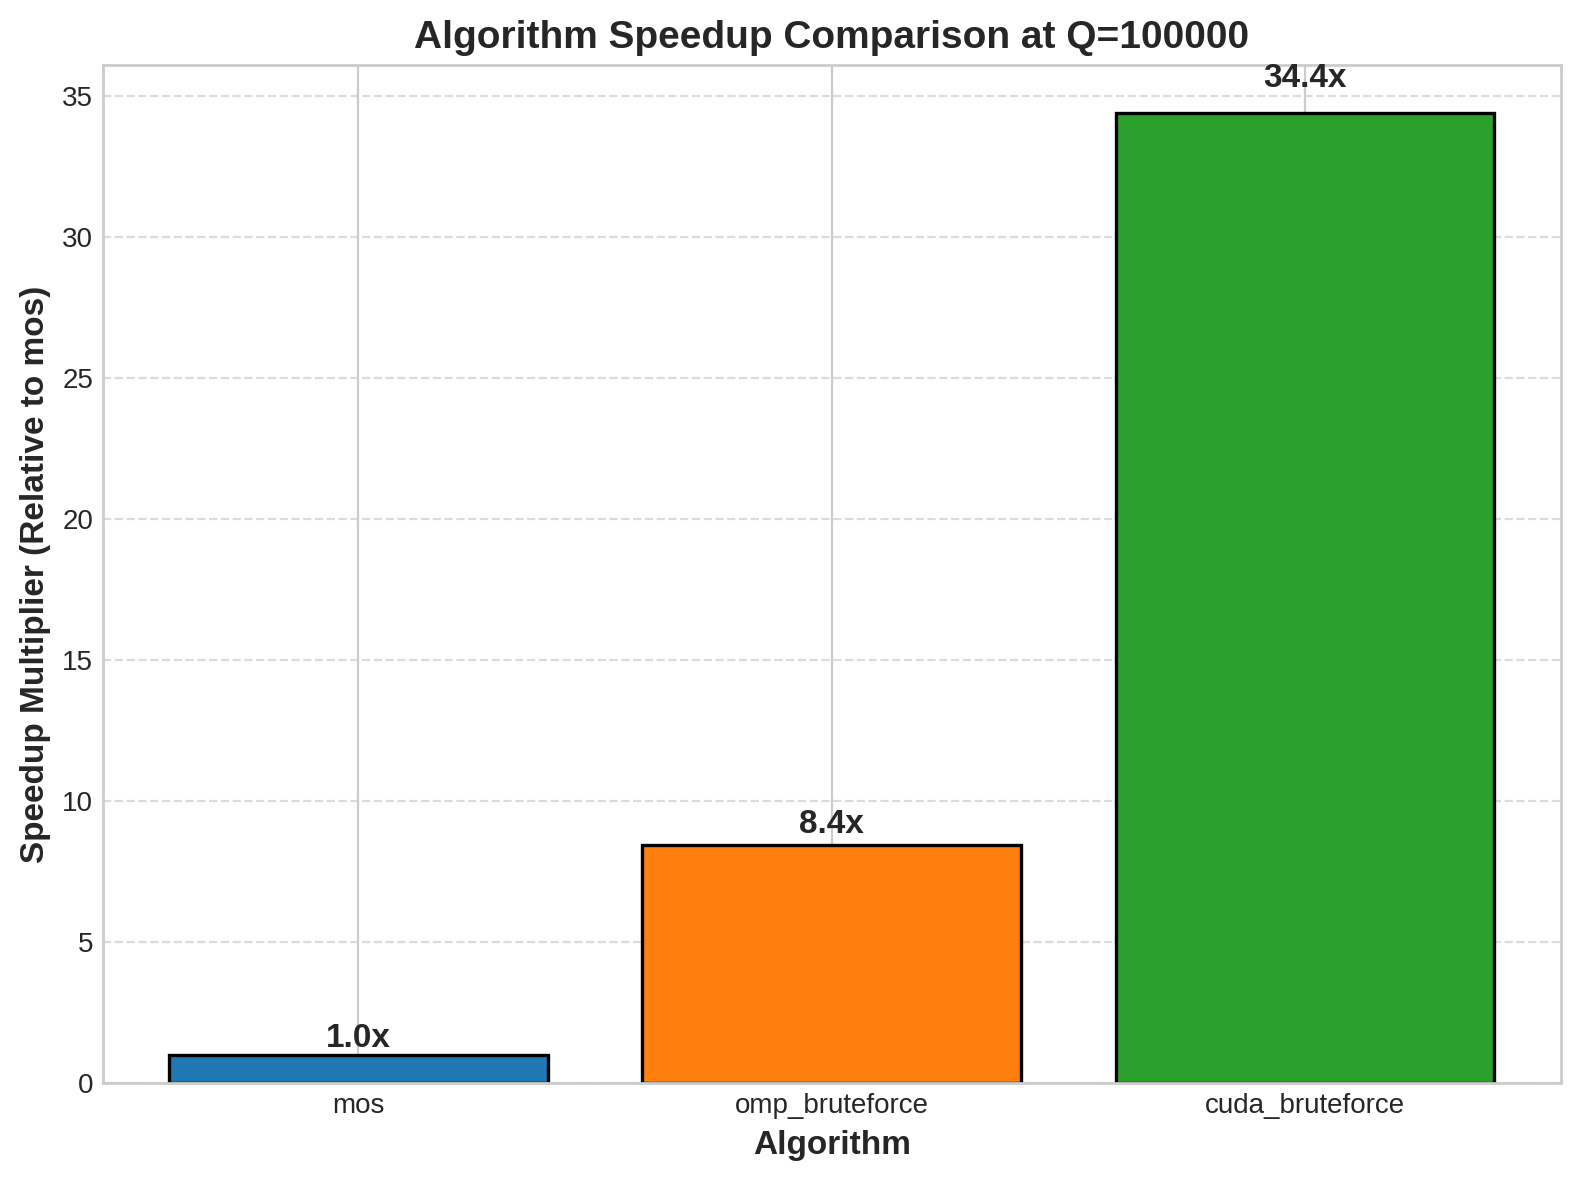
\includegraphics[width=0.9\linewidth]{plots/relative_speedup_bar.png}
   	\caption{Speedup comparison at $Q=100{,}000$ (medium ranges).}
   	\label{fig:speedup-bar}
   \end{figure}
   
   \begin{figure}[h!]
   	\centering
   	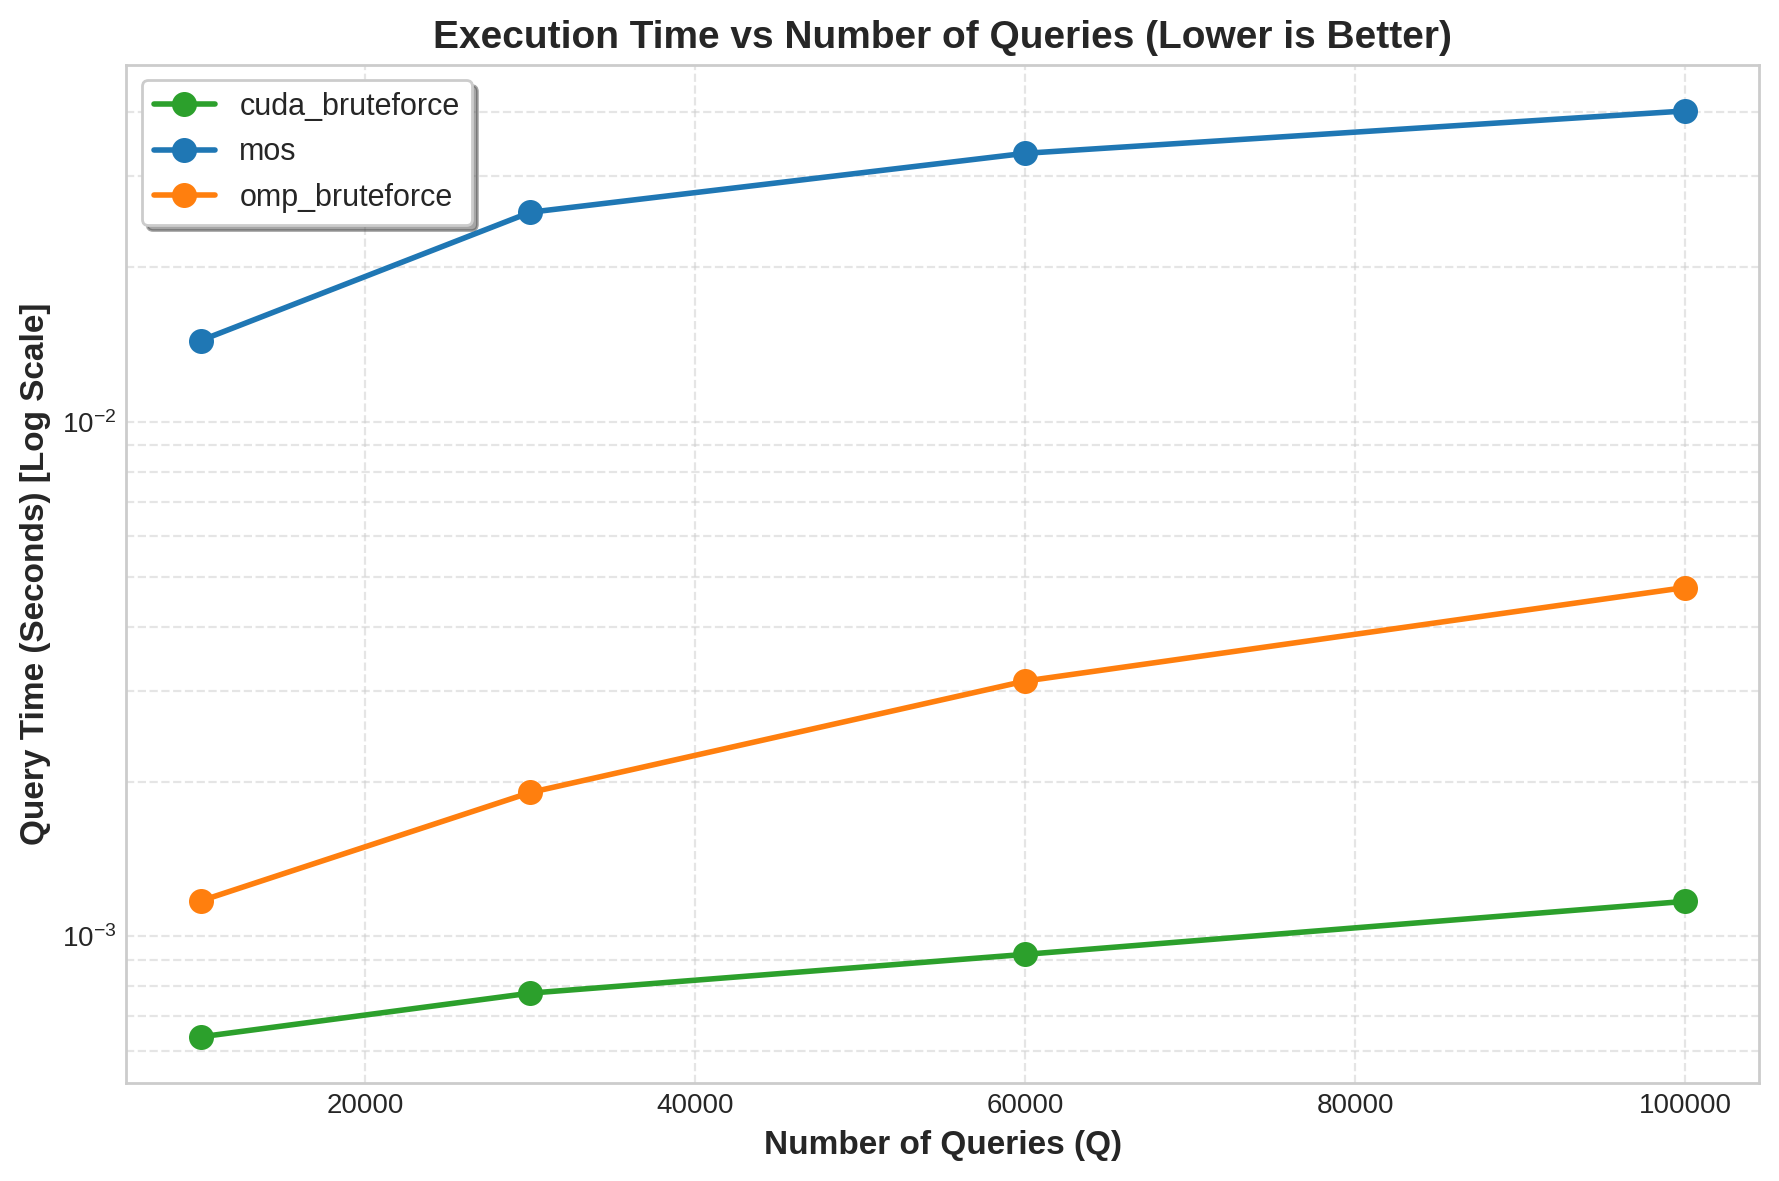
\includegraphics[width=0.9\linewidth]{plots/execution_time_vs_queries_log.png}
   	\caption{Execution time vs. number of queries (log scale).}
   	\label{fig:exec-time}
   \end{figure}
   
   \begin{figure}[h!]
   	\centering
   	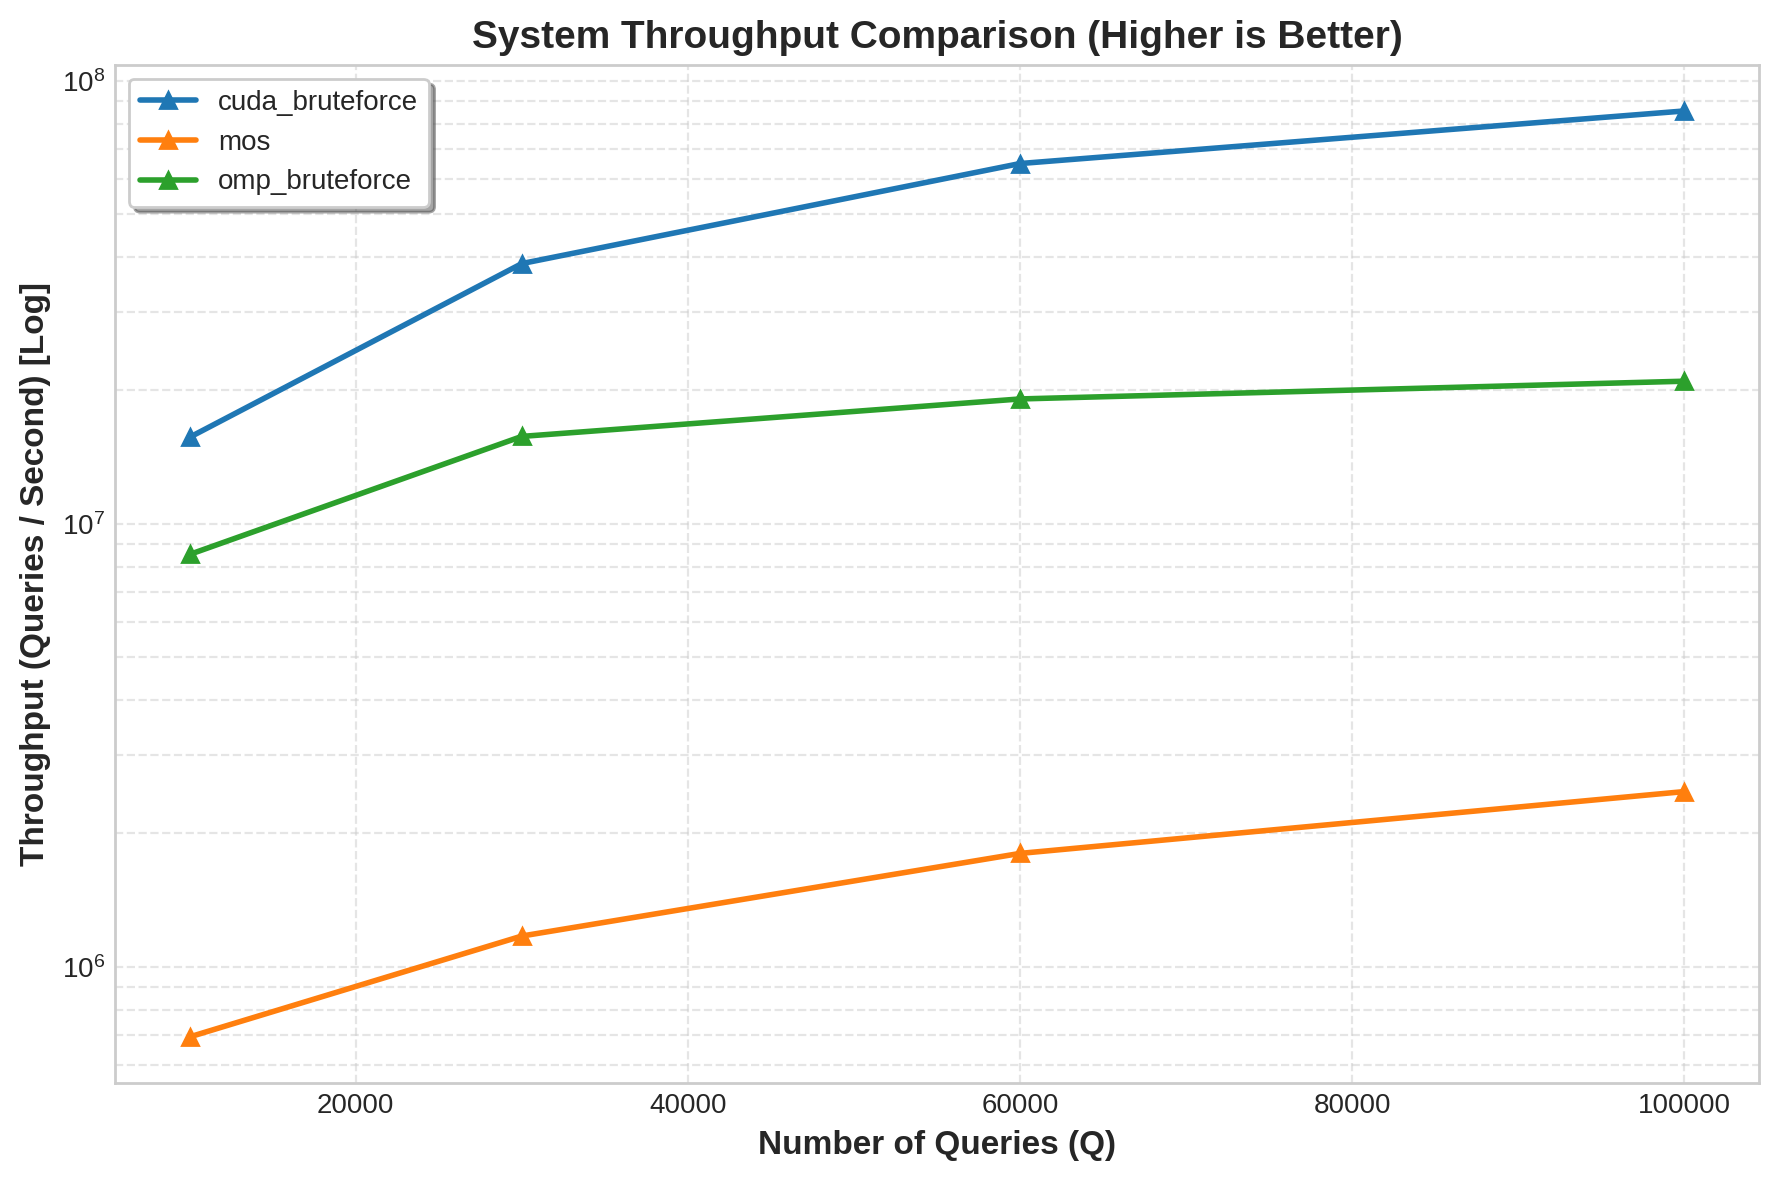
\includegraphics[width=0.9\linewidth]{plots/throughput_comparison_log.png}
   	\caption{Throughput comparison across methods (log scale).}
   	\label{fig:throughput}
   \end{figure}
   
   \begin{figure}[h!]
   	\centering
   	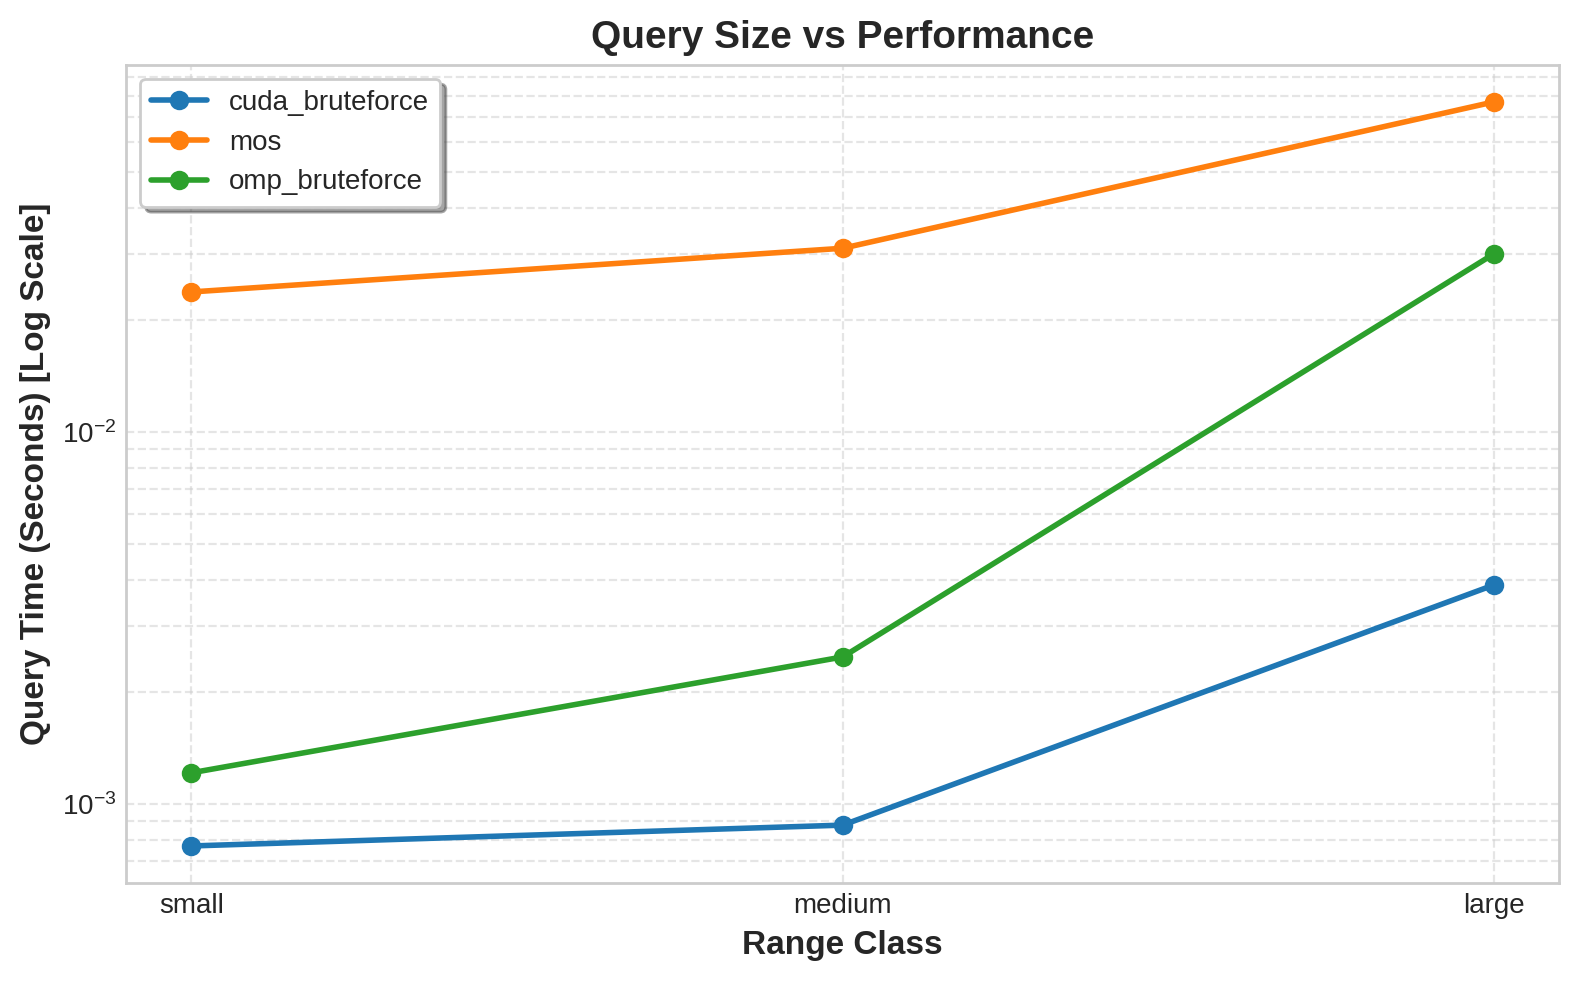
\includegraphics[width=0.85\linewidth]{plots/query_size_vs_performance_log.png}
   	\caption{Query size vs. performance across range classes.}
   	\label{fig:range-perf}
   \end{figure}
   
   \begin{figure}[h!]
   	\centering
   	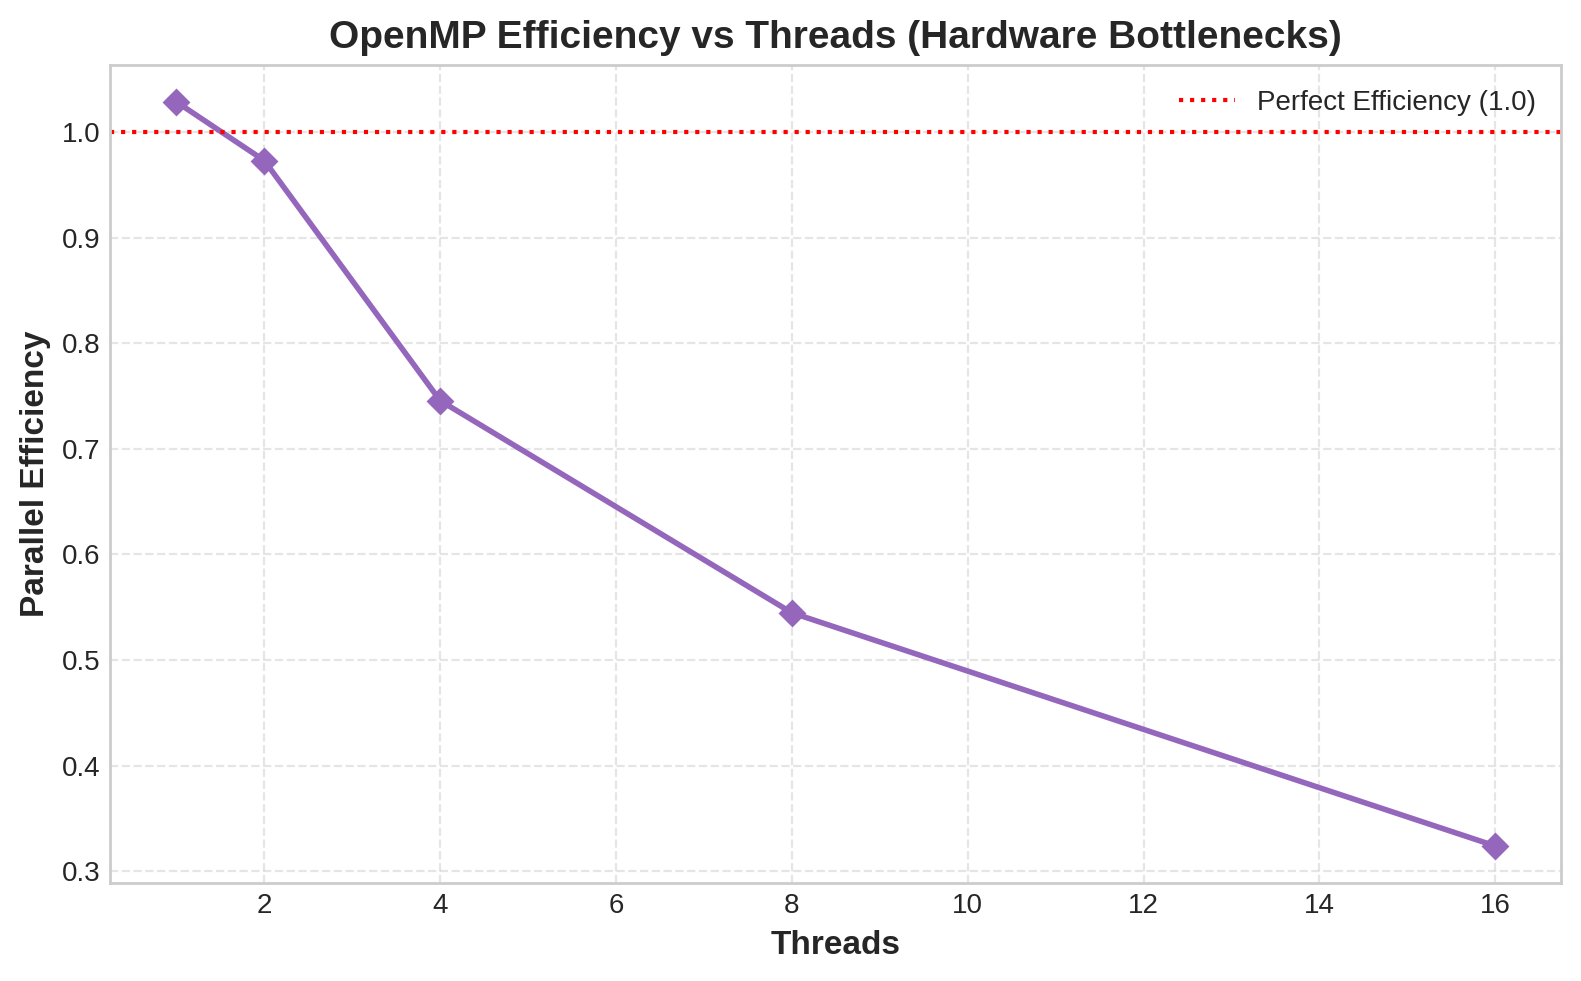
\includegraphics[width=0.85\linewidth]{plots/efficiency_vs_threads.png}
   	\caption{OpenMP efficiency vs. thread count.}
   	\label{fig:omp-eff}
   \end{figure}

%	%\chapter
	\clearpage
	\addcontentsline{toc}{section}{References}
	\bibliographystyle{IEEEtran}
	\bibliography{mybib}
	% to add references to TOC without section numbering
  
     \end{document}
%        
%       
